
Diese Hypothese geht davon aus, dass sich der Schnee bei mechanische Anregung von einem festen in den flüssigen Zustand übergeht. Je nach dem wie hoch der LWC ist, findet dieser Übergang statt oder nicht.

Um die Idee zu testen, wird ein vibrierendes Objekt mit hoher Dichte auf den Schnee gelegt, und es wird beobachtet, wie sich das Objekt durch den Schnee bewegt.

Die Form des Objekts wurde vom AvaNode übernommen.  Ein Name, analog zum AvaNode, ist VibraNode. Für die Umsetzung wurde ein Morphologischer Kasten mit drei Varinanten erstellt.


\begin{figure}[H]
    \centering
    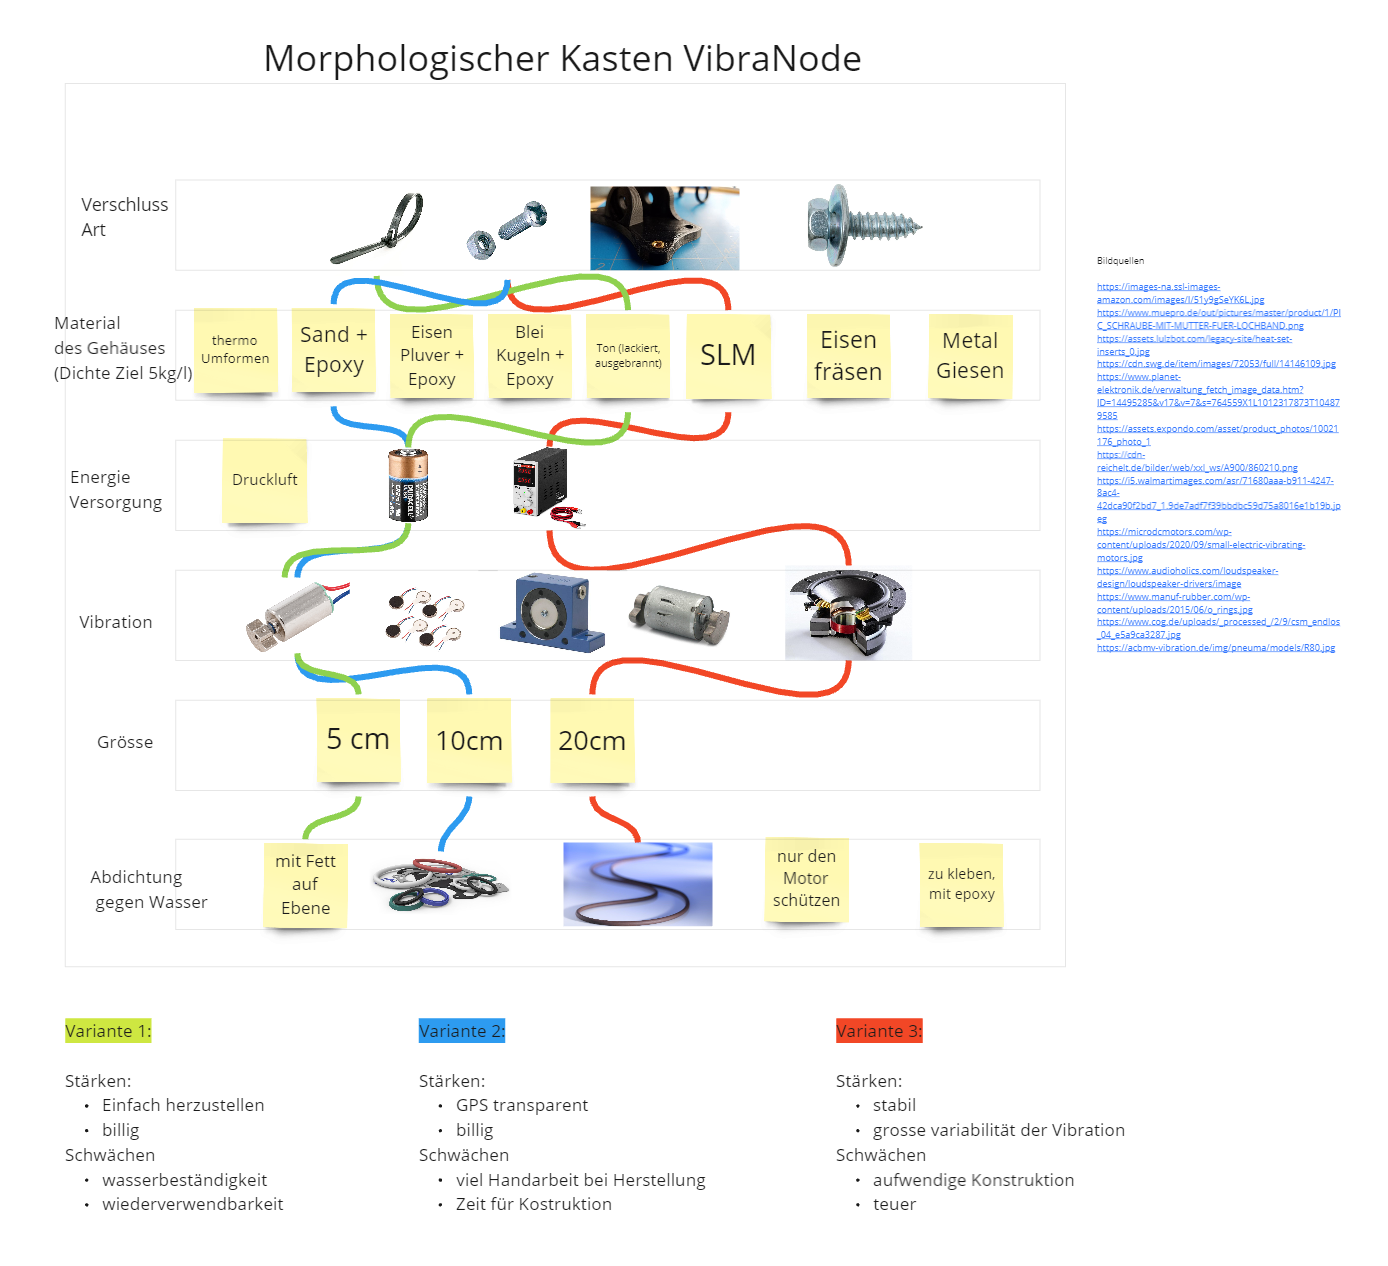
\includegraphics[width=0.8\textwidth]{Bilder/Unbenann2t.PNG}
    \caption{Morphologischer Kasten für VibraNode}
    \label{fig:Bildverarbeitnugskonzpet}
\end{figure}


Variante 1 wurde gewählt, da die Umsetztung und das Testen einfach ist. Die Schwächen, besonders die Wiederverwendbarkeit, sind hier in der Vorstudie noch nicht gravierend.

Die Testergebnisse fielen negativ aus. Der VibraNode konnte trotz seiner Dichte von 1600 kg/m3 nicht in den Schnee eindringen. Auch wenn der Schnee wurde mit flüssigem Wasser gesättigt war. Damit  stellt sich die neue Frage, ob der LWC einen kausalen oder nur einen korrelativen Zusammenhang mit Gleitschneelawinen hat, und wie weit die Vorgeschichte des Schnees mitbetrachtet werden muss. \cite{Altman.2015}
